\section{Scan Performance and Time graphs}
\label{sec:performance}

\subsection{Scan Performance}

How the rack's behaviour during a run shaped its spectrum (Figure~\ref{fig:performance}).
With \app{Analyse each run as it ends} ticked, each run is analysed as it closes; any other
is chosen under \app{Dataset} (the refresh button looks for new runs, the folder button
takes one from anywhere) and shown on every tab by \app{Show and analyse}.

Every check gives PASS, WARN, FAIL or N/A with the number it decided on; the
\app{Verdict} is the worst, with the line's width and what moved it. A deviation is flagged
only when it is both improbable under counting statistics and large enough to matter
against the line's width. Select a check to read what it found.

\begin{description}
    \item[Voltage scan.] Hits tagged with a voltage other than their bunch's; the
        calibration as \denis{} fits it, and against earlier runs calibrated the same way;
        the HV during the scan against its calibration.
    \item[Timing.] Whether the loop kept up with the triggers, stalls and pauses (a sleeping
        PC shows here), bunches taken before their step settled, missed triggers, the TOF
        peak against its gate.
    \item[Beam and spectrum.] Beam losses and stability, the line's position scan by scan
        against what the HV and laser monitors predict, the spectrum's shape, each channel.
    \item[Sources.] The cooler as the analysis takes it, a rolling mean over
        \code{cooler: rolling\_s} (15\,s), how far the readings scatter about it, and
        whether each hit's own reading is what its ions saw; the laser through the Doppler
        shift.
    \item[Detectors.] Each PMT's afterpulsing: its counts within \code{dead\_time\_us} of
        its own beyond what the other PMTs show, its scatter across scans against dead
        time, and a dead time suggested for \denis{}, never applied.
\end{description}

\app{Flagged for review} lists what deserves a look, with its reason; nothing is cut.
\app{Systematic inputs} gives each source of error as a width at the line, in scan volts
and MHz, marked measured, declared (in the settings) or not yet known; the Monte Carlo
that turns them into errors is \denis{}'s. A short block goes to the ELOG as each run is
analysed; \app{Post systematics to ELOG} posts the whole table. \app{Export report} writes
\code{run\_NNNN\_performance.yaml} and \code{run\_NNNN\_systematics.yaml} beside the run.

\begin{figure}[ht]
    \centering
    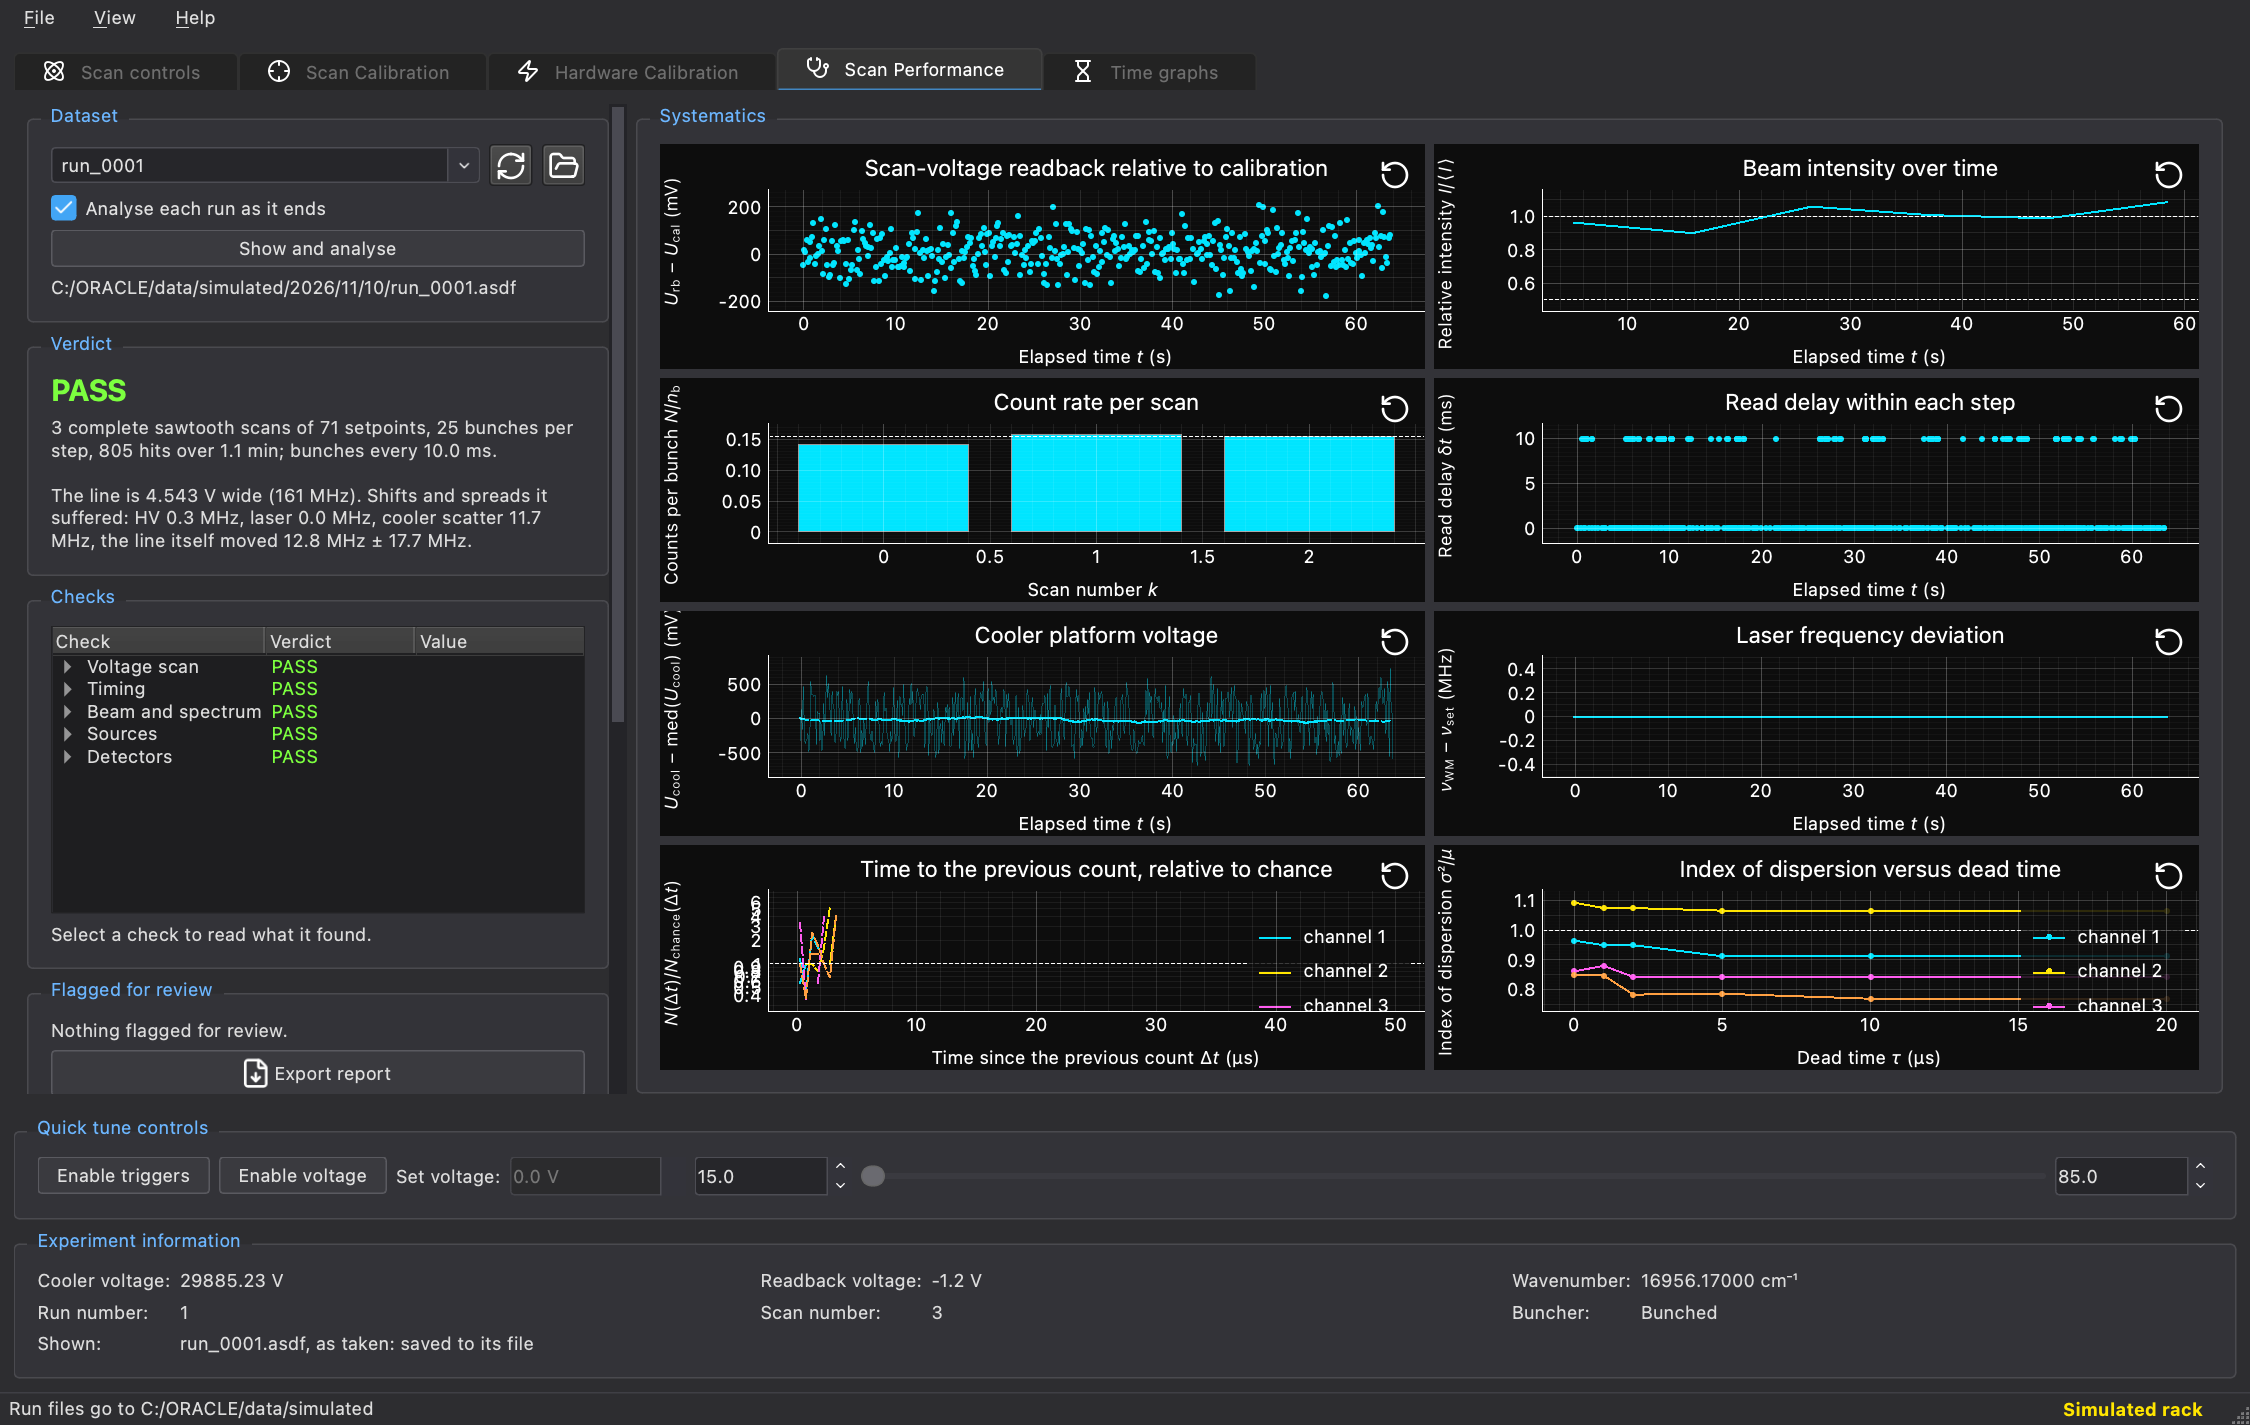
\includegraphics[width=\textwidth]{fig_performance_tab}
    \caption{\app{Scan Performance} for a simulated run: the verdict and checks, and a plot
        per systematic.}
    \label{fig:performance}
\end{figure}

\subsection{Time graphs}

Counts against time for the chosen channels, in bins of 100\,s down to 0.1\,s at the trigger
rate in force, to watch the beam. Below, each PMT's afterpulse ratio as data arrive: its
pairs within the dead time on itself over those on the others, 1 by chance, shown in the
warning colour above 2.
